\section{Data caching: concept, infrastructure and initiatives}
Simulations of caching layers based on reference WLCG workloads showed the ability to hide latency even when data is read for the first time. The simulations have been conducted using using XCache technology (from the xrootd software framework \cite{xroot}).

It should be noticed that Within the root framework \cite{root} it is also possible to cache data from the client side while the file starts to be accessed, this is usually as as reading ahead. Read ahead ability is very effective for low latencies and enables the remote reading option for sites close to the main source of the data, the Data Lake and enables sites to opt for an storage-less approach. For moderate to high network latencies the impact of Round Trip Time (RTT) start to be noticeable and CPU inefficiencies grow with the the increasing latency.\\
In WLCG there are around 160 facilities spread worldwide contributing to the global storage and computing infrastructure. The sites has different roles and scopes, they may supporting different experiments and many of them have local scientific communities. Among these many sites there is big variety on network topologies and hence a wide range of network performance metrics. The working group is investigating how to enable storage-less or state-less storage approach for sites that are interested mainly in processing facilities without the burden to operate and maintain a full fledged storage system. These sites will use the Data Lake as the main source of data and will access these data via caches (state-less approach) or remote access (storage-less approach) form their data processing facilities.

%The new models for distributed computing together with the Data Lake concept will open the opportunity for sites accessing data from all sites from Data Lake. 
%An example could be a relatively small Tier-2 currently providing storage and computing 
%to WLCG experiments, needing to maintain a storage system which is of little use to them. If this site is close 
%enough to a the Data Lake they could consider about accessing data remotely, and if they are on a more distant 
%(in network latency units) place they could interface with data by deploying a stateless storage as a caching 
%layer for latency hiding and eventual file reusability. 
In Fig. \ref{datalake-sketch} is shown a tentative 
sketch envisioning a Data Lake composed by sites and federations holding the bulk of the data regions, and 
the different types of computing-oriented sites, commercial clouds and HPCs accessing the Data Lake.\\

\begin{figure}
  \centering
  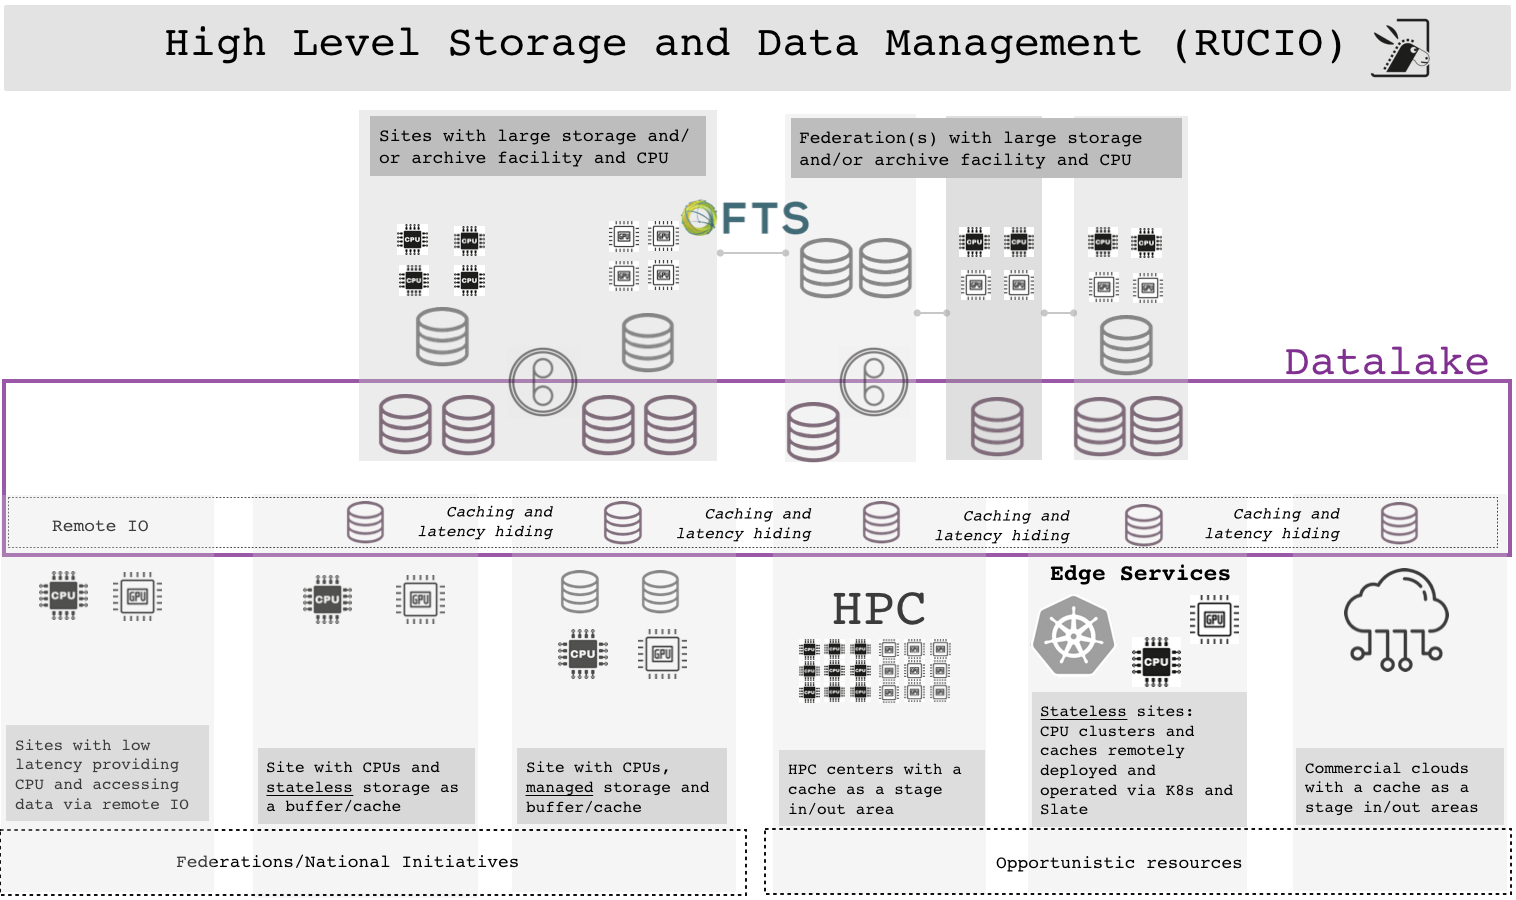
\includegraphics[height=7.8cm]{datalake-sketch-square.png}
  \caption{{\em (center)} Data Lake sketch composed by sites and federations holding the bulk of the data regions, and the different types of computing-oriented sites, commercial clouds and HPCs accessing the Data Lake }
  \label{datalake-sketch}
\end{figure}
The working group has promoted the deployment of several caching models to operate in a region and on a site level. We are investigating three different approaches: a) High performance caching servers in US to feed a region Southern California (SoCal) and Chicago; and b) caching federation to feed data to regional sites (as in Italy); and c) a site caching mechanism as state-less Tier-2 storage (Munich and Birmingham). The results obtained confirm that caching is a promising mechanism to address the analysis challenge and help increasing an efficient usage of the storage and hence able to optimize the overall cost, still meeting the
HL-LHC data storage needs. The caching layer setup at SoCal demonstrates that three sites (Riverside, Caltech and San Diego) can benefit from a common caching layer of 1~PB (c.f. with the old model where the site had to deal with 5~PB of stateful storage installation), this cache can serve 90\% of the jobs/user request at 1/5th of the cost in hardware and alleviating the site to manage a complex storage service.\\
The initiative in LMU Munich demonstrated that an old disk pool node, with a simple hardware configuration (JBOD) and simple XCache deployment could serve up to 3k concurrent jobs of ATLAS workflows reading data from the neighbour site in Hamburg (DESY) and from a far site in China (IHEP in Beijing). The test concluded that the difference in CPU efficiency when reading from the neighboring site and from the far site is no longer a showstopper taking into account the distance and the latency (Fig. ~\ref{lmu-xcache}).\\

\begin{figure}[h]
  \centering
  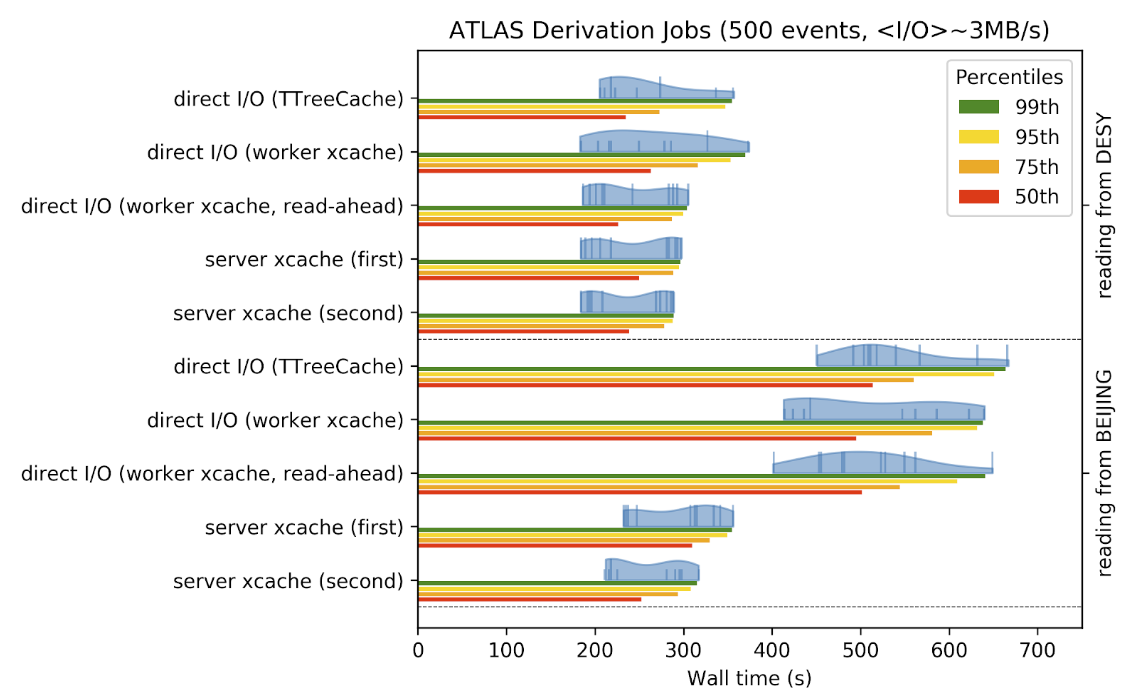
\includegraphics[height=6.5cm]{lmu-xcache.png}
  \caption{{\em (center)} XCache running on modest hardware at LMU. Successfully served 3.2k analysis and derivation jobs from ATLAS with and average I/O of 1~MB/s and 3~MB/s respectively. Effective latency hiding is achieved for high latency data consumption.}
  \label{lmu-xcache}
\end{figure}




